\documentclass[letterpaper]{article}
\usepackage[submission]{aaai2027}
\usepackage[hyphens]{url}
\usepackage{graphicx}
\urlstyle{rm}
\def\UrlFont{\rm}
\usepackage{natbib}
\usepackage{caption}
\frenchspacing
\setlength{\pdfpagewidth}{8.5in}
\setlength{\pdfpageheight}{11in}
\usepackage{booktabs}
\usepackage{amsmath}
\usepackage{multirow}
\pdfinfo{/TemplateVersion (2027.1)}
\setcounter{secnumdepth}{0}
\renewcommand{\thetable}{S\arabic{table}}
\renewcommand{\thefigure}{S\arabic{figure}}

\title{Supplementary Document\\
\large Use LLMs to Build Repair Tools, Not Patch Generation:\\Cost-Effective
Automated Program Repair}
\author{Anonymous submission}
\affiliations{}

\begin{document}
\maketitle

\noindent This document carries what the main paper's page budget could not.
Nothing here introduces a claim the paper does not already make: each item is
the tabular or graphical form of a number the Results section gives, or a
measurement the paper cites without room to print. Assignment ids (R1--R5,
C1--C6), the arm names, and every metric definition are the main paper's.
Values are generated from \texttt{results/} by the released scripts
(\texttt{run.py tables}, \texttt{run.py figures}); none is transcribed.

\section{Where the Repairs Come From}

Table~\ref{tab:source} decomposes every repair by the strategy that produced
it, with the mean patch each leaves and whether it carries a misconception
label, pooled over both builders. Shares are over repaired submissions; the LLM
row belongs to \textsc{CoEP}\textsubscript{LF} and sits outside that
denominator. The last rows are the framework-only ablation, the identical tool
with the builder's rules removed, which is the same artifact under either
builder because nothing the model wrote survives in it.

\begin{table}[h]
\centering\small\setlength{\tabcolsep}{5pt}
\begin{tabular}{lrrc}
\toprule
Repair source & share (\%) & mean RPS & labelled \\
\midrule
1. rules & 24.6 & 0.100 & $\bullet$ \\
2. reference transplant & 75.4 & 0.581 & -- \\
\midrule
3. LLM (\textsc{CoEP}\textsubscript{LF}) & 8.2 & 0.724 & -- \\
\midrule
\multicolumn{4}{l}{\emph{Framework-only ablation (builder rules removed),}}\\
\multicolumn{4}{l}{\emph{first column is RR (\%) rather than share}}\\
\quad ablated & 98.69 & 0.492 & -- \\
\quad full tool & 99.06 & 0.463 & -- \\
\bottomrule
\end{tabular}

\caption{Repair source, patch size, and labelling, with the framework-only
ablation.}
\label{tab:source}
\end{table}

\section{What Escalation Costs, Assignment by Assignment}

The main paper reports the escalation rate $e$ as a corpus figure. It is not
uniform: Table~\ref{tab:cost} gives it per assignment alongside the calls it
implies, the local CPU each submission spends, and the one-off build wall
clock. Two readings matter for a department sizing this. The assignments that
escalate most are the ones whose local patches are largest rather than the
hardest ones, and the compute is not free: 5{,}940 submissions cost 4.8 core
hours of local search, on top of roughly 22 minutes of build per assignment per
builder. Neither figure appears in the dollar totals, which price model tokens
alone.

\begin{table}[h]
\centering\small\setlength{\tabcolsep}{5pt}
\begin{tabular}{lrrrr}
\toprule
& $e$ (\%) & calls & $\mathrm{ATT}_{\mathrm{cpu}}$ (s) & build (min) \\
\midrule
R1 & 0.7 & 8 & 2.28 & 32 \\
R2 & 22.5 & 196 & 3.18 & 27 \\
R3 & 0.0 & 0 & 1.83 & 18 \\
R4 & 9.2 & 66 & 3.43 & 28 \\
R5 & 0.9 & 2 & 4.79 & 18 \\
C1 & 13.2 & 116 & 3.17 & 20 \\
C2 & 23.3 & 261 & 2.22 & 38 \\
C3 & 13.0 & 18 & 6.94 & 3 \\
C4 & 5.3 & 4 & 1.34 & 12 \\
C5 & 15.6 & 24 & 4.86 & 4 \\
C6 & 66.7 & 4 & 6.58 & 6 \\
\midrule
\textbf{All} & \textbf{11.8} & \textbf{699} & \textbf{2.88} & \textbf{206} \\
\bottomrule
\end{tabular}

\caption{Escalation rate, calls, local CPU per submission, and build wall clock
per assignment, over both builders.}
\label{tab:cost}
\end{table}

\section{Robustness}

Table~\ref{tab:robust} puts three axes side by side: assignment difficulty, the
choice of builder, and the escalation threshold. The difficulty bands group the
eleven assignments as CS1, Codeforces 800--1000, and Codeforces 1200--2000, the
last folding C6's three submissions in rather than reporting them alone.

\begin{table}[h]
\centering\footnotesize\setlength{\tabcolsep}{1pt}
\begin{tabular}{lccc}
\toprule
& Refactory & PyDex & \textsc{CoEP}\textsubscript{LF} \\
Stratum & \multicolumn{3}{c}{RR (\%) / RPS} \\
\midrule
\multicolumn{4}{l}{\emph{Difficulty} (Sonnet builder)}\\
\quad CS1 (Refactory) & 90.8 / 0.397 & 98.6 / 0.382 & 99.4 / 0.269 \\
\quad CF 800--1000 & 83.1 / 0.663 & 99.4 / 0.942 & 100.0 / 0.572 \\
\quad CF 1200--2000 & 54.5 / 0.815 & 100.0 / 0.800 & 100.0 / 0.689 \\
\midrule
\multicolumn{4}{l}{\emph{Builder}}\\
\quad Claude Sonnet 5 & -- & 99.0 / 0.598 & 99.7 / 0.398 \\
\quad GPT-5.4-mini & -- & 98.9 / 0.669 & 99.7 / 0.411 \\
\midrule
\multicolumn{4}{l}{\emph{Threshold}, 29 measured settings}\\
\quad range & -- & -- & 99.7 / 0.378--0.451 \\
\quad spend & \multicolumn{3}{c}{\$12.47--\$15.61 total} \\
\bottomrule
\end{tabular}

\caption{Difficulty, builder, and escalation threshold.}
\label{tab:robust}
\end{table}

Figure~\ref{fig:gate} plots every measured threshold setting against the
baselines it is compared to. The point is the emptiness between the cluster and
the baselines: the whole family spans \$12.47--\$15.61 of total spend, so which
setting ships cannot change a conclusion. The shipped rule, escalate a passing
local patch whose $\mathrm{RPS}$ exceeds 1, is marked with a star and is the
canonical run rather than the sweep's reconstruction of it.

\begin{figure}[h]
\centering
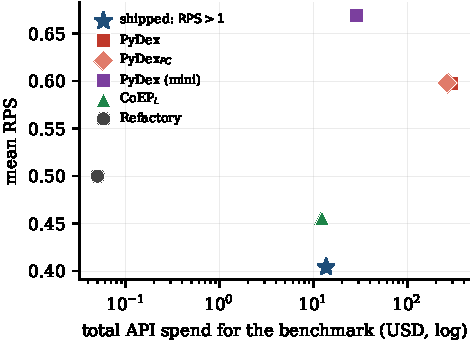
\includegraphics[width=\columnwidth]{figures/fig_gate.pdf}
\caption{Mean RPS against total spend. Each small marker is one threshold
setting; the star is the shipped rule. Repair rate is identical across all of
them.}
\label{fig:gate}
\end{figure}

\section{Rule Provenance}

The builders wrote 127 rules that fired, 1{,}216 times between them, against
the five always-on rules that fired 631 times. The distinction that matters is
reuse. Exactly one builder-written rule fired on more than one assignment,
\texttt{add\_missing\_call\_parens}, while \texttt{generic\_flip\_compare}
alone fired 455 times across 10 of the 11 assignments. The authored layer is
assignment-specific by construction, which is why it is priced per assignment
and the always-on layer is not.

The rules that carry the most submissions read as misconceptions rather than as
patches: \texttt{slice\_case\_check\_to\_equality} (115 repairs on C2),
\texttt{append\_missing\_return\_len\_after\_loop} (114 on R1),
\texttt{count\_compare\_relax} (112 on R2), and
\texttt{strict\_one\_should\_be\_exactly\_one} (96 on R2). On C4 a single rule,
\texttt{carry\_fix\_two\_value\_print}, repairs 27 of the assignment's 38
submissions under \texttt{claude-sonnet-5}.

The eight rules self-learning absorbed read the same way:
\texttt{counter\_var\_confusion}, \texttt{uniqueness\_count\_gt1\_to\_neq1},
\texttt{index\_vs\_count\_and\_uncalled\_bool} and
\texttt{missing\_else\_false} on R2 with \texttt{claude-sonnet-5};
\texttt{count\_equality\_for\_uniqueness},
\texttt{count\_uniqueness\_instead\_of\_direct\_membership} and
\texttt{missing\_call\_and\_predicate\_fix} on R2 with
\texttt{gpt-5.4-mini}; and \texttt{binarysearch\_zero\_exit} on C3.

\section{Reproducibility}

The repository contains the harness, every prompt, the 22 synthesized
repairers with their build costs, and the per-submission event log each arm
wrote. Four commands regenerate every number in both documents from those logs
without touching a model: \texttt{run.py tables}, \texttt{run.py figures},
\texttt{run.py numbers}, which recomputes each quantity and reports whether the
string still occurs in the paper, and \texttt{run.py stats}. The measured
threshold settings are archived as \texttt{results/threshold\_sweep.json}.

Two dependencies are outside our control and worth stating. Both builders are
closed commodity models reached through their providers' APIs, so a rebuild
cannot be guaranteed to reproduce the same rules; what is released is the tools
those builds produced, which are ordinary Python and run offline. Refactory's
replication package is its authors' and is cloned rather than vendored.

\end{document}
